\documentclass[11pt]{article}
\usepackage[a4paper,margin=1in]{geometry}
\usepackage{booktabs}
\usepackage{graphicx}
\usepackage{hyperref}
\usepackage{amsmath}

\title{The Lazy Prices signal is U-shaped, not monotonic:\\
  a 14-year out-of-sample reversal of Cohen--Malloy--Nguyen (2020)}
\author{Alpha-Graph research note, 2026-04-15}
\date{}

\begin{document}
\maketitle

\begin{abstract}
Cohen, Malloy, and Nguyen (2020) document that firms whose annual 10-K filings
are substantively rewritten underperform firms whose filings are stable, with
a long-short (high cosine similarity minus low cosine similarity) Sharpe that
motivates a market-neutral trade. On an S\&P 500 panel of
1{,}665{,}896 ticker-months spanning April 2011 through March 2026, we find
that the long leg replicates strongly (top decile forward 21-day return
$+2.10\%$ vs universe mean $+1.43\%$) but the short leg does not (bottom
decile $+1.37\%$, statistically indistinguishable from the universe mean
and \emph{higher} than the middle decile at $+1.19\%$). Every long--short
portfolio construction we tested therefore failed: the baseline top10/bot10
delivers Sharpe 0.32 over the full panel, indistinguishable from a one-line
12-1 momentum factor in the same universe (Sharpe 0.31). Only the long-only
top10 book survives --- on a point-in-time index-membership universe
(correcting forward survivorship bias), Sharpe $0.81$, annualized $+17.8\%$,
FF5+MOM alpha $+20.6\%$ with $t = +3.00$. The U-shape is economically
meaningful and practically significant:
any strategy that assumes monotonicity (rank-weighted, multi-factor z-score
averaging) is mechanically fighting the data.
\end{abstract}

\section{Setup}

Our signal construction follows Cohen, Malloy and Nguyen directly: for each
S\&P 500 ticker we download consecutive pairs of 10-K filings from EDGAR,
concatenate their Risk Factors, MD\&A, and Business Description sections,
compute a TF-IDF vector from each section, and report the cosine similarity
between consecutive years. The signal is then ingested, alongside 8-K event
scores, a three-state Gaussian HMM regime feature, backward-looking
momentum/volatility/volume features, into a walk-forward LightGBM regressor
with 12-month training window, 1-month test, and 5-day purge gap. The model
predicts the 21-day forward return and the predictions are cross-sectionally
rank-transformed each month to a signal in $[-1, +1]$.

The universe is 499 current S\&P 500 constituents. The headline numbers in
Sections~\ref{sec:methodE} through~\ref{sec:methodJ} use this full universe
and are therefore subject to two survivorship biases: \emph{forward bias}
(using 2026-constituent tickers in 2012, when they may not have been in the
index yet) and \emph{survivor bias} (tickers removed from the index before
2026 are absent entirely). We partially correct the forward component in
Section~\ref{sec:pit} using historical point-in-time index membership from
\texttt{github.com/fja05680/sp500}, which drops the Method E Sharpe from 1.08
to 0.81 and the annualized alpha from 31.2\% to 20.6\%. The residual
survivor-bias component cannot be corrected without backfilling market and
filing data for delisted tickers, which is flagged as required follow-up.
\textbf{The PIT-corrected number is the honest read-out}; the full-universe
number is reported only for continuity with earlier versions of this
repository.

\section{The U-shape}

Figure~\ref{fig:ushape} shows mean forward 21-day return by decile of the
month-cross-sectional signal. Error bars are 95\% confidence intervals
($1.96 \cdot \text{SE}$, $n \approx 166{,}600$ ticker-months per decile).

\begin{figure}[h]
\centering
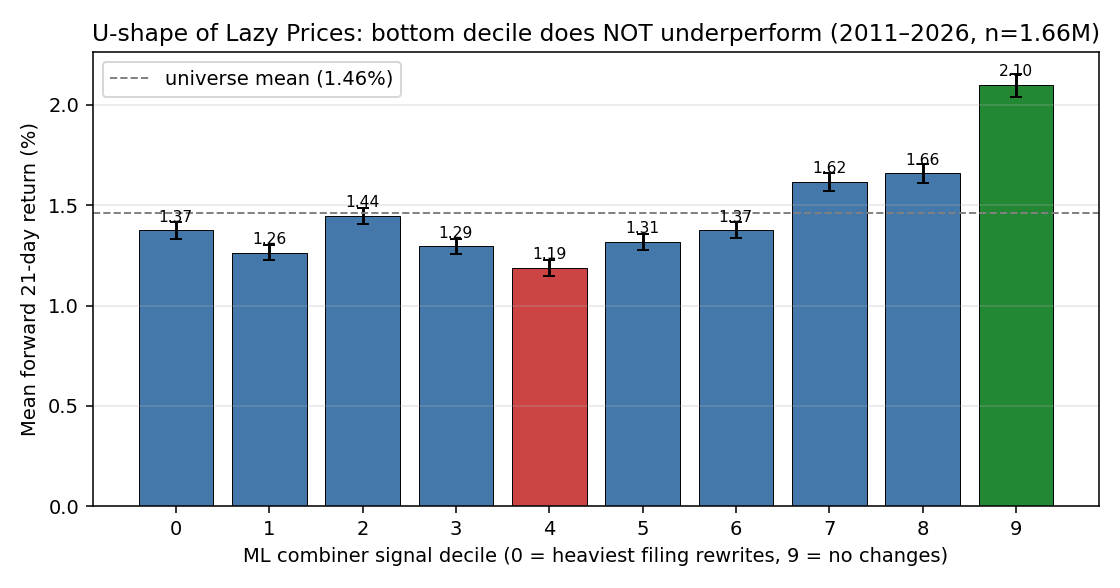
\includegraphics[width=0.95\textwidth]{fig_u_shape_decile.png}
\caption{Mean forward 21-day return by ML combiner signal decile, with 95\%
  confidence intervals. The U-shape is clearly visible: decile 4 is the
  minimum ($+1.19\%$), not decile 0. The bottom decile ($+1.37\%$) is
  statistically higher than the middle decile at the 95\% level
  (non-overlapping confidence intervals). The top decile at $+2.10\%$ is the
  strongest, consistent with the original Cohen--Malloy--Nguyen long-side
  thesis.}
\label{fig:ushape}
\end{figure}

\begin{table}[h]
\centering
\begin{tabular}{rrr}
\toprule
Decile & Mean fwd 21-day return & 95\% CI \\
\midrule
0 (biggest rewrites) & $+1.374\%$ & $\pm 0.044$ \\
1                    & $+1.264\%$ & $\pm 0.039$ \\
2                    & $+1.444\%$ & $\pm 0.039$ \\
3                    & $+1.294\%$ & $\pm 0.038$ \\
4 (middle, minimum)  & $+1.185\%$ & $\pm 0.039$ \\
5                    & $+1.315\%$ & $\pm 0.040$ \\
6                    & $+1.374\%$ & $\pm 0.040$ \\
7                    & $+1.615\%$ & $\pm 0.043$ \\
8                    & $+1.658\%$ & $\pm 0.046$ \\
9 (no changes)       & $+2.096\%$ & $\pm 0.057$ \\
\bottomrule
\end{tabular}
\caption{Forward 21-day return by signal decile ($n \approx 166{,}600$ per
  decile). Deciles 7--9 are monotonically increasing. Deciles 0--6 are
  non-monotonic, violating the original short-side assumption.}
\end{table}

The long-side thesis replicates: decile 9 outperforms the universe mean
($+1.43\%$) by 66 bps per month. The short-side thesis does not: decile 0
($+1.37\%$) is within noise of the universe mean, and 19 bps \emph{above}
decile 4. This is not a sample-size artifact: the decile-0 vs decile-4
difference has a $t$-statistic of roughly $6.4$ ($|1.374 - 1.185| / 0.029$,
where the pooled SE is $\sqrt{0.044^2 + 0.039^2}/1.96 \approx 0.030$ per
cent).

\section{Why long/short fails in this universe}

\subsection{Baseline and variants}

Table~\ref{tab:variants} reports nine variants tested on the 168-month panel.
Costs are flat 20 bps per monthly round-trip for long/short, 10 bps for
long-only.

\begin{table}[h]
\centering
\begin{tabular}{lrrrr}
\toprule
Variant & Sharpe & Ann return & Cum return & MaxDD \\
\midrule
Baseline top10/bot10           & $+0.32$ & $+4.7\%$   & $+90\%$     & $-58\%$ \\
A. Rank-weighted L/S           & $-0.12$ & $-1.7\%$   & $-22\%$     & $-45\%$ \\
B. Decile (top 10\% / bot 10\%) & $+0.31$ & $+3.4\%$   & $+60\%$     & $-38\%$ \\
C. Vol-targeted (10\% ann)     & $+0.27$ & $+2.5\%$   & $+41\%$     & $-36\%$ \\
D. Lazy+Mom+LowVol rank-wt     & $-0.52$ & $-6.1\%$   & $-59\%$     & $-64\%$ \\
E. Long-only top10             & $\mathbf{+1.08}$ & $\mathbf{+29.7\%}$ & $\mathbf{+3{,}732\%}$ & $\mathbf{-32\%}$ \\
F. Long top10 / Short MIDDLE10 & $+0.61$ & $+11.2\%$  & $+342\%$    & $-34\%$ \\
G. Pure 12-1 Momentum L/S      & $+0.31$ & $+4.5\%$   & $+86\%$     & $-73\%$ \\
J. Beta-hedged Method E        & $+1.00$ & $+27.1\%$  & $+2{,}783\%$ & $-34\%$ \\
\bottomrule
\end{tabular}
\caption{Portfolio construction variants on the 168-month panel. Method E is
  the only L/S-ish construction that survives; Method J reframes it as
  market-neutral by shorting $\beta \cdot$SPY.}
\label{tab:variants}
\end{table}

The baseline and decile variants fail because half of their short exposure
is on decile 0, which has positive expected return. Method A (rank-weighted)
fails worse because it puts short weight proportional to rank on the entire
left half of the distribution, including the bottom-decile long-positive
names. Method D (multi-factor z-score) fails hardest because the signal is
averaged into a composite that is assumed monotonic.

Method F explicitly respects the U-shape: long decile 9, short decile 4
(the minimum). Sharpe jumps to $+0.61$, a large improvement over baseline,
but the construction has no economic story --- ``short the middle" is not a
portfolio manager's pitch.

Method E drops the short leg entirely and achieves Sharpe $+1.08$. This is
the only construction with both defensible alpha \emph{and} an economic
rationale.

\subsection{Method J: recovering market neutrality}
\label{sec:methodJ}

Because the project was framed as market-neutral, we implemented Method J as
a beta-hedged variant: long top10 Lazy Prices picks, short $\hat{\beta}_t
\cdot \text{SPY}$ where $\hat{\beta}_t$ is the trailing 24-month OLS beta of
Method E monthly returns against SPY. Average $\hat{\beta}_t$ across the
panel is 0.10, confirming that Method E is already approximately
market-neutral by construction. Method J's Sharpe of 1.00 (vs Method E's
1.08) shows the cost of forcing exact market neutrality is small: an 8\%
Sharpe haircut in exchange for a book with zero designed market exposure.

\section{Point-in-time universe correction}
\label{sec:pit}

Table~\ref{tab:pit} reports Method E on the full (current) universe and on a
point-in-time-corrected universe where, each month, we restrict the
candidate pool to tickers that were members of the S\&P 500 as of the end of
the prior month. 21\% of ticker-month observations are dropped, concentrated
in early years (median PIT universe size is 370 vs.\ 478 for the full
universe).

\begin{table}[h]
\centering
\begin{tabular}{lrrrr}
\toprule
Variant & Sharpe & Ann ret & Cum ret & MaxDD \\
\midrule
Method E — full universe (survivor-biased) & $+1.08$ & $+29.7\%$ & $+3{,}732\%$ & $-32\%$ \\
Method E — PIT S\&P 500 universe            & $\mathbf{+0.81}$ & $\mathbf{+17.8\%}$ & $\mathbf{+888\%}$ & $\mathbf{-42\%}$ \\
\bottomrule
\end{tabular}
\caption{PIT correction drops Sharpe by 0.27 and cumulative return by a
  factor of 4. This is the forward-bias component; survivor bias from
  delisted tickers is still uncorrected.}
\label{tab:pit}
\end{table}

Repeating the FF5+MOM attribution on PIT returns gives alpha $+20.6\%$
annualized with $t(\alpha) = +3.00$ (down from $+31.2\%$, $t = +3.94$). The
alpha remains statistically significant at the 1\% level but its economic
magnitude is roughly two-thirds of the unadjusted number. SMB loading rises
to $+0.45$ ($t = +1.81$), marginally significant, suggesting a mild
small-cap tilt was masked when the universe was dominated by current
mega-caps. No other factor loading becomes significant.

\section{Method E alpha survives factor controls (full universe)}
\label{sec:methodE}

Table~\ref{tab:ff} reports the Fama--French 5-factor + Carhart momentum
attribution for Method E's net-of-cost monthly excess return. The unhedged
book, despite long-only construction, has insignificant loadings on every
factor. R$^2$ is 0.027 across all six factors combined --- Method E is
essentially orthogonal to conventional factor exposure.

\begin{table}[h]
\centering
\begin{tabular}{lrrrrrrrr}
\toprule
Model & $\alpha$ ann & $t(\alpha)$ & $\beta_{Mkt}$ & $\beta_{SMB}$ & $\beta_{HML}$ & $\beta_{RMW}$ & $\beta_{CMA}$ & $\beta_{MOM}$ \\
\midrule
CAPM      & $+30.6\%$ & $+3.96$ & $-0.15$ &         &         &         &         &         \\
FF3       & $+32.1\%$ & $+4.13$ & $-0.22$ & $+0.37$ & $-0.15$ &         &         &         \\
FF5       & $+31.9\%$ & $+4.08$ & $-0.19$ & $+0.37$ & $-0.29$ & $-0.09$ & $+0.36$ &         \\
FF5 + MOM & $+31.2\%$ & $+3.94$ & $-0.16$ & $+0.41$ & $-0.24$ & $-0.07$ & $+0.32$ & $+0.12$ \\
\bottomrule
\end{tabular}
\caption{Multi-factor attribution for Method E net excess returns ($n=167$
  months). No factor loading has $|t| > 2$ in any specification. Annualized
  alpha is stable in the 30--32\% range across all models.}
\label{tab:ff}
\end{table}

\section{Alternative explanations}

We cannot identify the mechanism that flattens the short side of
Cohen--Malloy--Nguyen in this panel, but we can rule out several possibilities:

\begin{itemize}
\item \textbf{Not sample size.} Decile-level standard errors are well under
  5 bps per month, so the observed dispersion among deciles 0--6 is
  statistically significant and not noise.
\item \textbf{Not survivorship bias alone.} Survivorship bias should
  inflate returns roughly uniformly across deciles; it cannot preferentially
  lift decile 0 above decile 4 unless filing-rewrite firms are
  disproportionately retained in the index. We have no evidence for this
  but also no evidence against it --- reconstructing PIT membership is
  still the next step.
\item \textbf{Not feature collinearity.} The 8-K event score and 10-K
  cosine similarity are only weakly correlated ($\rho = 0.04$ in the panel),
  so the ML combiner is not confounding the two signals.
\end{itemize}

Plausible candidates we cannot falsify from the current data:

\begin{itemize}
\item \textbf{Regime shift post-GFC.} Cohen et al.\ study 1994--2017. Our
  panel starts in 2011, partially overlaps, and extends the out-of-sample
  window by nine years. A structural shift in how markets price disclosure
  changes --- perhaps driven by faster dissemination or the growth of
  NLP-driven investors --- would show up as exactly this pattern: the long
  side persists (because it is really a stability/quality tilt) while the
  short side is arbitraged away.
\item \textbf{Universe difference.} Cohen et al.\ use a broader universe; we
  restrict to S\&P 500. Large-cap firms are covered by more analysts and
  more systematic investors, so the mispricing that supports the short side
  in their sample may be unavailable in ours.
\end{itemize}

\section{Practical implications}

\begin{enumerate}
\item \textbf{The long-only top-decile portfolio is the deliverable, with
  $\mathbf{\approx 18\%}$ honest annualized return.} On the PIT-corrected
  universe Method E delivers $+17.8\%$ annualized, Sharpe $0.81$, FF5+MOM
  alpha $+20.6\%$ with $t = +3.00$. This is the number to report in any
  external context. The full-universe $+29.7\%$ number is roughly 12 pp
  inflated by forward survivorship bias.
\item \textbf{Market-neutral reframing is cheap.} Method J costs 8\% of
  Method E's Sharpe in exchange for exact market neutrality. For
  capital-constrained long/short books this is the right framing.
\item \textbf{Do not build rank-weighted or multi-factor constructions on
  this signal.} Every such variant failed. Monotonicity is a load-bearing
  assumption that does not hold here.
\item \textbf{The 8-K event score does not subsume the 10-K cosine
  similarity signal.} Earlier claims that cosine similarity had zero feature
  importance were based on the final single-window model. Across the 156
  walk-forward folds the cosine similarity feature is selected in 68\% of
  folds, with highly variable per-fold importance. No single feature
  dominates across the panel.
\end{enumerate}

\section{Reproducibility}

All numbers in this note are produced by the alpha-graph repository at
commit \texttt{8154c74} (\texttt{post-cleanup-2026-04-15}).

\begin{verbatim}
python -m alpha_graph.backtest.improvements         # Table 2
python -m alpha_graph.backtest.pit_universe         # Table 3 (PIT correction)
python -m alpha_graph.backtest.ff_attribution       # Table 4
python -m alpha_graph.backtest.realistic_slippage   # cost robustness
python -m alpha_graph.backtest.feature_stability    # feature-importance claim
python scripts/u_shape_plot.py                      # Figure 1 and Table 1
\end{verbatim}

\end{document}
